\secnumbersection{Validación de la solución}


% Se debe validar la solución propuesta. Esto significa probar o demostrar que la solución propuesta es válida para el entorno donde fue planteada.

% Tradicionalmente es una etapa crítica, pues debe comprobarse por algún medio que vuestra propuesta es básicamente válida. En el caso de un desarrollo de software es la construcción y sus pruebas; en el caso de propuestas de modelos, guías o metodologías podrían ser desde la aplicación a un caso real hasta encuestas o entrevistas con especialistas; en el caso de mejoras de procesos u optimizaciones, podría ser comparar la situación actual (previa a la memoria) con la situación final (cuando la memoria está ya implementada) en base a un conjunto cuantitativo de indicadores o criterios.

% \subsection{EJEMPLO DE COMO CITAR TABLAS}

% Se colocó una tabla que se puede referenciar también desde el texto (Ver tabla \ref{table:coloquios}).

% \begin{table}[h]
%     \centering
%     \caption{\label{table:coloquios} Coloquios del Ciclo de Charlas Informática.} Fuente: Elaboración Propia.
%     \begin{tabular}{|p{7cm}|p{7cm}|}
%         \hline
%         Título Coloquio & Presentador, País \\
%         \hline
%         ``Sensible, invisible, sometimes tolerant, heterogeneous, decentralized and interoperable... and we still need to assure its quality...''' & Guilherme Horta Travassos, Brasil.\\
%         \hline
%         ``Dispersed Multiphase Flow Modeling: From Environmental to Industrial Applications''' & Orlando Ayala, EE.UU.\\
%         \hline
%         ``Líneas de Producto Software Dinámicas para Sistemas atentos el Contexto''' & Rafael Capilla, España.\\
%         \hline
%         ... & ... \\
%         \hline
%     \end{tabular}
% \end{table}

% \subsection{Implementación}

\subsection{Stack de tecnologías}

En primera instancia existe la tentación por implementar una modificación completa de la herramienta \textit{MESHER\_GENERATOR}, esto es viable pero se descarta cuando se prioriza la escalabilidad y mantenibilidad de código. Sobre la eficiencia y rapidez de la propuesta, que son características importantes que evidencian calidad, se evaluarán en secciones posteriores.
En \textit{MESHER\_GENERATOR} sólo se realizarán las modificaciones descritas en las secciones anteriores que incluyen funcionalidades para identificar y exportar los Octantes a refinar, para generar estadísticas al finalizar el refinamiento en las mallas y las pequeñas modificaciones a las funcionalidades de exportación de la información de los Octantes para luego identificarlos globalmente y así refinar los Octantes correctos.

Entonces, como debemos ejecutar \textit{MESHER\_GENERATOR}, existen varias formas de realizar esto, pero se escogerá la que utilice menos recursos para ejecutar llamadas a sistema como lo hace \textit{bash} en linux. Ya que se requiere de funcionalidades básicas como iteraciones y manipulación de archivos, esta es una buena herramienta a utilizar.

\subsection{Proceso de análisis}

Para validar la propuesta, se utilizará una serie de mallas con diferentes complejidades.
\begin{itemize}
    \item Malla de corteza cerebral con área de refinamiento prismática en la zona frontal.

        Propuesta inicial, de por sí la malla de corteza cerebral posee una complejidad media, contiene algunas zonas cóncavas que podrían complejizar el refinamiento. El prisma se posicionará en la zona del lóbulo frontal.
    \item Malla de corteza cerebral con área de refinamiento prismática en la zona trasera.

        En la zona trasera, lóbulo occipital de la corteza cerebral, de naturaleza cóncava e irregular se posicionará el prisma para refinar localmente, esto con el fin de complejizar el trabajo del algoritmo.
    \item Malla de Moai con área de refinamiento prismática en la zona superior.

        Para este análisis se escogió una representación de un Moai, que naturalmente no posee múltiples zonas cóncavas, entonces se aplicará el área de refinamiento en la zona superior donde se presenta la mayor cantidad de zonas cóncavas. 
    \item Malla de Moai con área de refinamiento prismática en la zona inferior.

        Se utilizará también la zona inferior, que no posee mayor nivel de complejidad respecto a su concavidad, con motivo de aumentar el universo de soluciones.
    \item Malla de paladar con área de refinamiento prismática en la zona superior.

        Esta representación posee áreas muy finas con respecto a el resto de la malla, entonces se aplicó un área de refinamiento adicional en la zona superior por su complejidad en función de concavidad.
    \item Malla de coxis.

        En general esta representación es muy compleja, presenta zonas muy pequeñas y con múltiples concavidades.
\end{itemize}

A cada una de estas mallas se les aplicará el algoritmo propuesto con un threshold cero y cien iteraciones como cota superior. 
Luego de iterar las mallas, se analizará sus estadísticas sobre Elementos de mala calidad.

\subsection{Ejecución}

En cada malla dependiendo de su complejidad se aplicará o no, un área prismática para refinar localmente, de esta manera añadir consistencia a los resultados.

La única malla a la que no se le aplicará el área prismática es la malla de coxis debido a su compleja naturaleza explicada en la sección anterior.

\subsubsection{Malla de corteza cerebral}

Al implementar el algoritmo propuesto en la malla de corteza cerebral, entregándole como input el threshold definido en esta propuesta, el modelo de la corteza, el modelo de la superficie prismática a refinar, la base de nombre de los archivos exportados y una cota de cien iteraciones.  Obtenemos el siguiente output \ref{out:cortex_1}, que nos muestra un identificador de cada iteración con la cantidad de Octantes a refinar al finalizar dicha iteración, finalizando exitosamente en la cuarta iteración con una malla sin elementos inválidos y reduciendo la cantidad de Octantes a refinar casi de manera exponencial.

Luego se ejecutó el algoritmo con la zona a refinar en el lóbulo occipital con el siguiente output \ref{out:cortex_2}.

Si bien, en esta ocasión se logró obtener una malla válida con algunas iteraciones adicionales, la cantidad de Elementos inválidos se comporta similar a el caso anterior.


\begin{lstlisting}[style=Console,caption={Output de ejecución algoritmo propuesto en malla de corteza cerebral con zona a refinar en lóbulo frontal.\\ Fuente: Elaboración propia.},label={out:cortex_1}]
input  >    ./script.sh 0.0 ./data/cortex.mdl ./data/cortex_surf_roi.mdl c_5r7 100
output >    Threshold: 0.0
            Main surface: ./data/cortex.mdl
            Reference surface: ./data/cortex_surf_roi.mdl
            Base name: c_5r7
            Number of iterations: 100
            Octants to improve in iteration 0: 21
            Octants to improve in iteration 1: 7
            Octants to improve in iteration 2: 2
            Octants to improve in iteration 3: 1
            No more Octants to improve in iteration 4.
\end{lstlisting}

\begin{lstlisting}[style=Console,caption={Output de ejecución algoritmo propuesto en malla de corteza cerebral con zona a refinar en lóbulo occipital.\\ Fuente: Elaboración propia.},label={out:cortex_2}]
input  >    ./script.sh 0.0 ./data/cortex.mdl ./data/cortex_surf_roi_2.mdl c_5r7_2 100
output >    Threshold: 0.0
            Main surface: ./data/cortex.mdl
            Reference surface: ./data/cortex_surf_roi_2.mdl
            Base name: c_5r7_2
            Number of iterations: 100
            Octants to improve in iteration 0: 52
            Octants to improve in iteration 1: 27
            Octants to improve in iteration 2: 11
            Octants to improve in iteration 3: 6
            Octants to improve in iteration 4: 7
            Octants to improve in iteration 5: 3
            No more Octants to improve in iteration 6.
\end{lstlisting}

\begin{figure}[!ht]
    \centering
    \begin{subfigure}[t]{0.45\textwidth}
        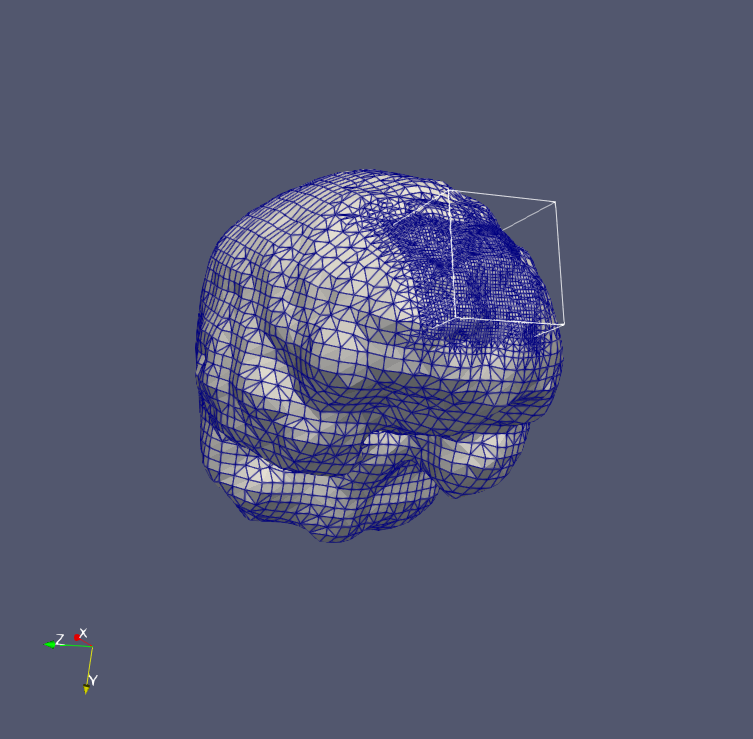
\includegraphics[width=1.0\textwidth]{figures/meshes/c_5r7_01.png}
        \caption{Representación corteza cerebral con refinamiento en lóbulo frontal.}
    \end{subfigure}
    \begin{subfigure}[t]{0.45\textwidth}
        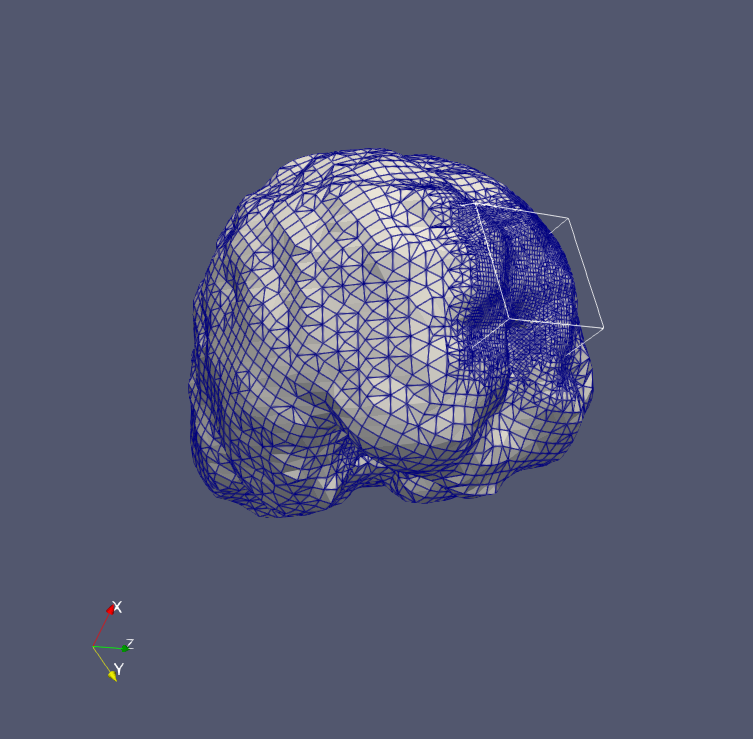
\includegraphics[width=1.0\textwidth]{figures/meshes/c_5r7_2_01.png}
        \caption{Representación corteza cerebral con refinamiento en lóbulo occipital.}
    \end{subfigure}
    \caption{ Diferentes localidades de refinamiento en corteza cerebral. }
    Fuente: Elaboración propia.
    \label{fig:c_5r7_all}
\end{figure}


\subsubsection{Malla de Moai}

La ejecución del algoritmo en la malla de Moai para los casos con refinamiento inferior y superior, como podemos ver en \autoref{out:moai_1} y \autoref{out:moai_2}, respectivamente. En ambos casos se logró una malla válida en aproximadamente 5 iteraciones, pero a diferencia de los casos anteriores, como la corteza cerebral y la zona inferior en el Moai, la malla de Moai en la zona superior, se comporta aumentando en un grado menor la cantidad de Octantes por refinar entre la primera y segunda iteración, luego disminuye la cantidad de Octantes manteniendo el aparente modelo exponencial.

\begin{lstlisting}[style=Console,caption={Output de ejecución algoritmo propuesto en malla de Moai con zona a refinar en zona inferior.\\ Fuente: Elaboración propia.},label={out:moai_1},float,floatplacement=H]
input  >    ./script.sh 0.0 ./data/moai.mdl ./data/moai_surf_roi.mdl moai_5r7 100
output >    Threshold: 0.0
            Main surface: ./data/moai.mdl
            Reference surface: ./data/moai_surf_roi.mdl
            Base name: moai_5r7
            Octants to improve in iteration 0: 22
            Octants to improve in iteration 1: 5
            Octants to improve in iteration 2: 2
            Octants to improve in iteration 3: 1
            Octants to improve in iteration 4: 1
            No more Octants to improve in iteration 5.
\end{lstlisting}


\begin{lstlisting}[style=Console,caption={Output de ejecución algoritmo propuesto en malla de Moai con zona a refinar en zona superior.\\ Fuente: Elaboración propia.},label={out:moai_2}, float,floatplacement=H]
input  >    ./script.sh 0.0 ./data/moai.mdl ./data/moai_surf_roi_2.mdl moai_5r7_2 100
output >    Threshold: 0.0
            Main surface: ./data/moai.mdl
            Reference surface: ./data/moai_surf_roi_2.mdl
            Base name: moai_5r7_2
            Number of iterations: 100
            Octants to improve in iteration 0: 10
            Octants to improve in iteration 1: 12
            Octants to improve in iteration 2: 9
            Octants to improve in iteration 3: 3
            No more Octants to improve in iteration 4.
\end{lstlisting}


\begin{figure}[!ht]
    \centering
    \begin{subfigure}[t]{0.45\textwidth}
        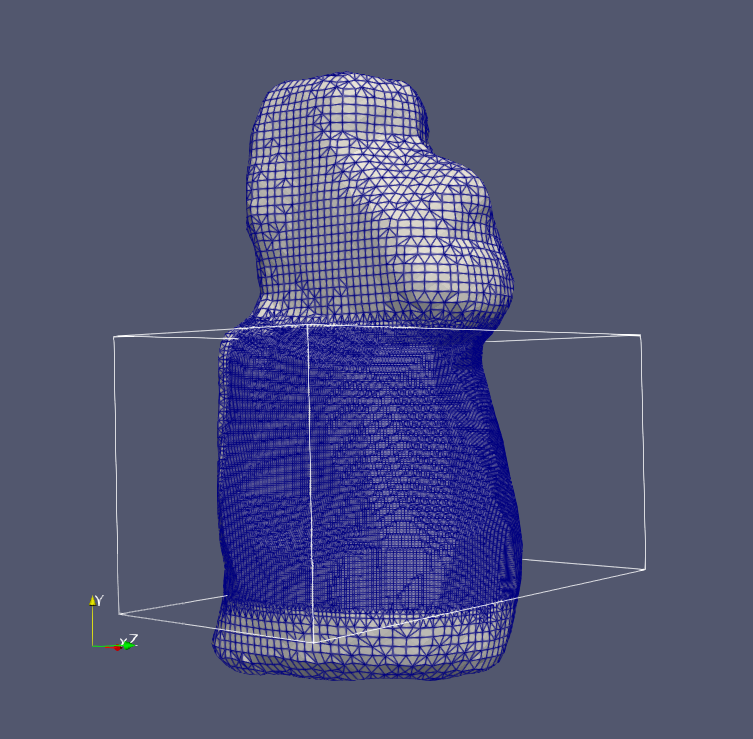
\includegraphics[width=1.0\textwidth]{figures/meshes/moai_5r7_01.png}
        \caption{Representación Moai con refinamiento en zona inferior.}
    \end{subfigure}
    \begin{subfigure}[t]{0.45\textwidth}
        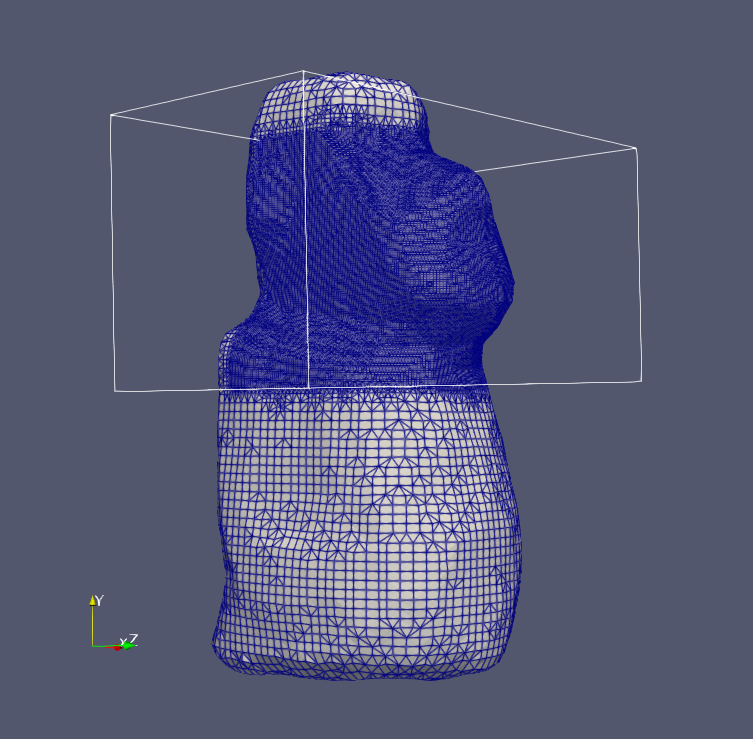
\includegraphics[width=1.0\textwidth]{figures/meshes/moai_5r7_2_01.png}
        \caption{ Representación Moai con refinamiento en zona superior. }
    \end{subfigure}
    \caption{ Diferentes localidades de refinamiento en Moai. }
    Fuente: Elaboración propia.
    \label{fig:moai_5r7_all}
\end{figure}

\subsubsection{Malla de paladar}


\begin{lstlisting}[style=Console,caption={Output de ejecución algoritmo propuesto en malla de Moai con zona a refinar en zona superior.\\ Fuente: Elaboración propia.},label={out:palate_1}, float,floatplacement=H]
input  >    ./script.sh 0.0 ./data/palate.mdl ./data/palate_surf_roi.mdl palate_5r7 100
output >    Threshold: 0.0
            Main surface: ./data/palate.mdl
            Reference surface: ./data/palate_surf_roi.mdl
            Base name: palate_5r7
            Number of iterations: 100
            Octants to improve in iteration 0: 33
            Octants to improve in iteration 1: 17
            Octants to improve in iteration 2: 6
            Octants to improve in iteration 3: 1
            Octants to improve in iteration 4: 1
            No more Octants to improve in iteration 5.
\end{lstlisting}



En el caso de la malla de paladar, podemos 

\begin{figure}[!ht]
    \centering
    \begin{subfigure}[t]{0.8\textwidth}
        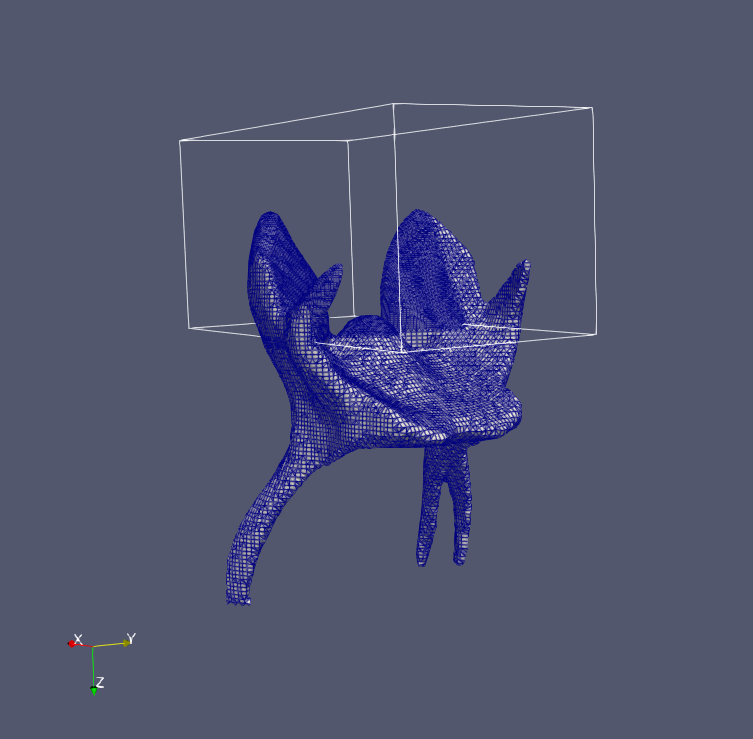
\includegraphics[width=1.0\textwidth]{figures/meshes/palate_5r7_01.png}
        % \caption{Representación Paladar con refinamiento en zona superior.}
    \end{subfigure}
    \caption{ Representación Paladar con refinamiento en zona superior. }
    Fuente: Elaboración propia.
    \label{fig:palate_5r7_all}
\end{figure}

\subsubsection{Malla de coxis}


\begin{lstlisting}[style=Console,caption={Output de ejecución algoritmo propuesto en malla de Moai con zona a refinar en zona superior.\\ Fuente: Elaboración propia.},label={out:moai_2}, float,floatplacement=H]
input  >    ./script.sh 0.0 ./data/palate.mdl ./data/palate_surf_roi.mdl palate_5r7 100
output >    Threshold: 0.0
            Main surface: ./data/palate.mdl
            Reference surface: ./data/palate_surf_roi.mdl
            Base name: palate_5r7
            Number of iterations: 100
            Octants to improve in iteration 0: 33
            Octants to improve in iteration 1: 17
            Octants to improve in iteration 2: 6
            Octants to improve in iteration 3: 1
            Octants to improve in iteration 4: 1
            No more Octants to improve in iteration 5.
\end{lstlisting}




\begin{figure}[!ht]
    \centering
    \begin{subfigure}[t]{0.8\textwidth}
        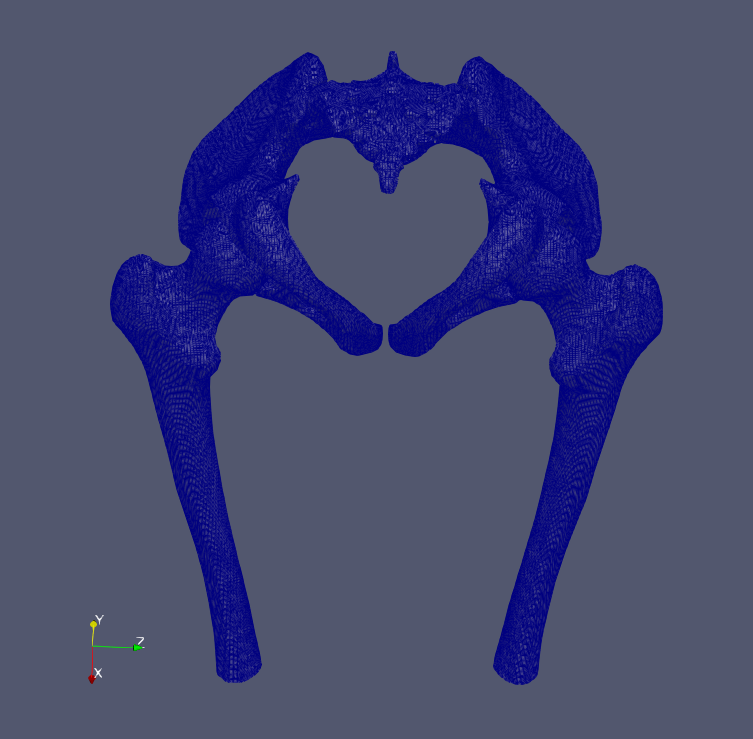
\includegraphics[width=1.0\textwidth]{figures/meshes/coxis_8r9_01.png}
    \end{subfigure}
    \caption{ Representación Coxis sin refinamiento local. }
    Fuente: Elaboración propia.
    \label{fig:coxis_8r9_all}
\end{figure}



\subsection{Resultados}

Para analizar el comportamiento del algoritmo, nos enfocaremos en ajustar la cantidad de iteraciones a algún modelo conocido, entregar una hipótesis sobre la anomalía en la malla del coxis y comparar con los resultados entregados en \cite{daines2018repairing}.

\subsubsection{Ajuste de la cantidad de iteraciones}

El algoritmo propuesto se comporta de muy buena manera para todas las mallas a excepción de la malla que representa el coxis, cuando logra converger, la cantidad de Octantes por refinar dando como resultado una malla válida, es posible reducir considerablemente la cantidad de Octantes por refinar en muy pocas iteraciones, a simple vista se podría entregar una hipótesis sobre el comportamiento del algoritmo en cada iteración.

Para esto, se considerará, a diferencia de lo que ya es tónica en lo antes mostrado, la cantidad de Elementos menores al threshold escogido, es decir, todos los Elementos que pertenecen a la malla y tienen $J_{ENS} \leq 0$, se denotará como $E_0$. Se elaboró la siguiente tabla con el $E_0$ en cada iteración para las diferentes mallas de los casos definidos, \autoref{table:num_els_ref}.

Lo evidente es la relación estrecha entre Elementos y Octantes que se respaldan en su naturaleza estructural. Luego, la aparente relación en el comportamiento de $E$ en todos los casos, permite comenzar la busqueda del modelo, por uno exponencial.


En la \autoref{table:num_els_ref} se muestra el comportamiento de $E_0$ en cada iteración, de aquí sólamente se analizarán los casos que convergen a cero.

\begin{table}[!ht]
\begin{tabular}{|lllllll|}
\hline
\multicolumn{7}{|c|}{Número de Elementos por refinar en cada iteración.}                                                                                                                                                                                                                    \\ \hline
\multicolumn{1}{|l|}{\textbf{N° Iteración}} & \multicolumn{1}{l|}{\textbf{cortex\_5r7}} & \multicolumn{1}{l|}{\textbf{cortex\_5r7\_2}} & \multicolumn{1}{l|}{\textbf{moai\_5r7}} & \multicolumn{1}{l|}{\textbf{moai\_5r7}} & \multicolumn{1}{l|}{\textbf{palate\_6r7}} & \textbf{coxis\_7} \\ \hline
\multicolumn{1}{|l|}{1}                     & \multicolumn{1}{l|}{27}                   & \multicolumn{1}{l|}{64}                      & \multicolumn{1}{l|}{26}                 & \multicolumn{1}{l|}{15}                 & \multicolumn{1}{l|}{25}                   & 242               \\ \hline
\multicolumn{1}{|l|}{2}                     & \multicolumn{1}{l|}{7}                    & \multicolumn{1}{l|}{32}                      & \multicolumn{1}{l|}{7}                  & \multicolumn{1}{l|}{12}                 & \multicolumn{1}{l|}{5}                    & 658               \\ \hline
\multicolumn{1}{|l|}{3}                     & \multicolumn{1}{l|}{2}                    & \multicolumn{1}{l|}{13}                      & \multicolumn{1}{l|}{2}                  & \multicolumn{1}{l|}{11}                 & \multicolumn{1}{l|}{3}                    & 435               \\ \hline
\multicolumn{1}{|l|}{4}                     & \multicolumn{1}{l|}{1}                    & \multicolumn{1}{l|}{6}                       & \multicolumn{1}{l|}{1}                  & \multicolumn{1}{l|}{3}                  & \multicolumn{1}{l|}{1}                    & 612               \\ \hline
\multicolumn{1}{|l|}{5}                     & \multicolumn{1}{l|}{0}                    & \multicolumn{1}{l|}{7}                       & \multicolumn{1}{l|}{1}                  & \multicolumn{1}{l|}{0}                  & \multicolumn{1}{l|}{1}                    & 679               \\ \hline
\multicolumn{1}{|l|}{6}                     & \multicolumn{1}{l|}{}                     & \multicolumn{1}{l|}{3}                       & \multicolumn{1}{l|}{0}                  & \multicolumn{1}{l|}{}                   & \multicolumn{1}{l|}{0}                    & 746               \\ \hline
\multicolumn{1}{|l|}{7}                     & \multicolumn{1}{l|}{}                     & \multicolumn{1}{l|}{0}                       & \multicolumn{1}{l|}{}                   & \multicolumn{1}{l|}{}                   & \multicolumn{1}{l|}{}                     & 880               \\ \hline
\multicolumn{1}{|l|}{8}                     & \multicolumn{1}{l|}{}                     & \multicolumn{1}{l|}{}                        & \multicolumn{1}{l|}{}                   & \multicolumn{1}{l|}{}                   & \multicolumn{1}{l|}{}                     & 1017              \\ \hline
\multicolumn{1}{|l|}{9}                     & \multicolumn{1}{l|}{}                     & \multicolumn{1}{l|}{}                        & \multicolumn{1}{l|}{}                   & \multicolumn{1}{l|}{}                   & \multicolumn{1}{l|}{}                     & 1179              \\ \hline
\multicolumn{1}{|l|}{10}                    & \multicolumn{1}{l|}{}                     & \multicolumn{1}{l|}{}                        & \multicolumn{1}{l|}{}                   & \multicolumn{1}{l|}{}                   & \multicolumn{1}{l|}{}                     & 1302              \\ \hline
\end{tabular}
\caption{ $E_0$ en cada iteración para los diferentes casos. }
\label{table:num_els_ref}
\end{table}

\subsection{Análisis de los resultados}

\subsubsection{ Análisis de la tasa de reducción de la cantidad de Elementos por refinar en cada iteración }

\begin{itemize}
    \item Definición de una secuencia exponencial.

    Para determinar si $E$ se comporta de manera exponencial, es esencial revisar cómo se comportan las reducciones entre cada par de números consecutivos y si sigue un patrón consistente con un modelo exponencial.

    Un modelo exponencial sigue la forma:
    $$y = a \cdot r^n$$
     
    donde:
    
    \begin{itemize}
        \item y es el valor en la n-ésima posición.
        \item a es el valor inicial (en nuestro caso, 21).
        \item r es la razón de reducción (un valor menor a 1).
        \item n es la posición en la secuencia.
    \end{itemize}
    
    Para verificar si una secuencia sigue un modelo exponencial, podemos examinar si el cociente entre cada par de términos consecutivos es aproximadamente constante. Es decir, si $\frac{y_{n+1}}{y_n}$ es constante.

    \item Cálculo del cociente entre términos consecutivos

    Calculamos el cociente entre cada par de números consecutivos en la secuencia de cada uno de los casos. \autoref{table:co_els_ref}

	\begin{table}[!ht]
	\begin{tabular}{|llllll|}
	\hline
	\multicolumn{6}{|c|}{ Cociente entre cantidad de Elementos por refinar consecutivos}                                                                                                                                                                           \\ \hline
	\multicolumn{1}{|l|}{\textbf{N° Iteración}} & \multicolumn{1}{l|}{\textbf{cortex\_5r7}} & \multicolumn{1}{l|}{\textbf{cortex\_5r7\_2}} & \multicolumn{1}{l|}{\textbf{moai\_5r7}} & \multicolumn{1}{l|}{\textbf{moai\_5r7}} & \textbf{palate\_6r7} \\ \hline
	\multicolumn{1}{|l|}{1-2}                   & \multicolumn{1}{l|}{0.259}          & \multicolumn{1}{l|}{0.500}             & \multicolumn{1}{l|}{0.269}         & \multicolumn{1}{l|}{1.25}         & 0.2             \\ \hline
	\multicolumn{1}{|l|}{2-3}                   & \multicolumn{1}{l|}{0.286}            & \multicolumn{1}{l|}{0.406}             & \multicolumn{1}{l|}{0.285}          & \multicolumn{1}{l|}{0.733}        & 0.6              \\ \hline
	\multicolumn{1}{|l|}{3-4}                   & \multicolumn{1}{l|}{0.500}            & \multicolumn{1}{l|}{0.462}              & \multicolumn{1}{l|}{0.5}            & \multicolumn{1}{l|}{0.273}         & 0.333            \\ \hline
	\multicolumn{1}{|l|}{4-5}                   & \multicolumn{1}{l|}{}                     & \multicolumn{1}{l|}{1.166}               & \multicolumn{1}{l|}{1.0}            & \multicolumn{1}{l|}{}                   & 1.0              \\ \hline
	\multicolumn{1}{|l|}{5-6}                   & \multicolumn{1}{l|}{}                     & \multicolumn{1}{l|}{0.429}               & \multicolumn{1}{l|}{}                   & \multicolumn{1}{l|}{}                   &                      \\ \hline
	\end{tabular}
	\caption{Cocientes entre cantidades de Elementos con $J_{ENS} \leq 0$ para los diferentes casos. }
	\label{table:co_els_ref}
	\end{table}


    \item Evaluación de los Cocientes.

    Para un modelo exponencial puro, los cocientes entre términos consecutivos deberán ser aproximadamente iguales. En este caso, los valores no lo son, pero están en un rango que sugiere una tendencia decreciente. Sin embargo, la variabilidad entre los cocientes da indicios de que la secuencia no se reduce de manera perfectamente exponencial con una sola razón común.

	Por ejemplo, en el caso de \textit{cortex\_5r7\_2}, sus cocientes se mantienen relativamente constante, aproximadamente $0.45$, a excepción del cociente en las iteraciones \textit{4-5} que se escapa casi al doble del promedio.


    \item Ajuste a un modelo exponencial

	Se ajustará a un modelo exponencial cada uno de los casos. Considerando $a_i$, valor inicial del caso $i$, se buscará una razón $r_i$ que mejor ajuste la reducción de la secuencia para el caso.
    
    Para esto, es necesario resolver la ecuación $$y = a_i \cdot r_{i}^{n}$$ para cada $n$ y encontrar el $r_i$ promedio que mejor describa la secuencia. Aunque los cocientes no son constantes, podemos ver si hay un $\bar{r_i}$ promedio que se ajuste razonablemente.

    \item Cálculo promedio geométrico

    El promedio geométrico de los cocientes es una manera de obtener una aproximación de la razón $\bar{r_i}$:

    Su valor se calcula en \autoref{table:r_fit}.

	\begin{table}[!ht]
 		\centering
		\begin{tabular}{|ll|}
		\hline
		\multicolumn{2}{|c|}{Promedio geométrico de los cocientes de cada caso}     \\ \hline
		\multicolumn{1}{|l|}{\textbf{Casos} $\mathbf{i}$}     & Promedio geométrico $\mathbf{\bar{r_i}}$ \\ \hline
		\multicolumn{1}{|l|}{cortex\_5r7}    & 0.333                                \\ \hline
		\multicolumn{1}{|l|}{cortex\_5r7\_2} & 0.542                                \\ \hline
		\multicolumn{1}{|l|}{moai\_5r7}      & 0.443                                \\ \hline
		\multicolumn{1}{|l|}{moai\_5r7\_2}   & 0.630                                \\ \hline
		\multicolumn{1}{|l|}{palate\_6r7}    & 0.408                                \\ \hline
		\end{tabular}
		\caption{Promedio geométrico de los cocientes de cada caso. }
		\label{table:r_fit}
	\end{table}

    Estos $\bar{r_i}$ indican que las secuencias podrían ajustarse aproximadamente por un modelo exponencial con razones cercanas a las propuestas en la tabla \ref{table:r_fit}.

    Gráficamente podemos ver el comportamiento de $E_0$ en cada iteración sobre los datos reales en \autoref{fig:exponential_fit_all}.  La gran mayoría de los casos se ajustan de buena manera, podríamos decir que el algoritmo se comporta bajo un modelo exponencial, sin considerar el caso excepcional del coxis.  A diferencia de los demás casos, la malla del coxis diverge también de manera exponencial.  Esto puede explicarse debido al comportamiento en cascada que tiene el algoritmo y la estructura continua de las vecindades cóncavas.
    
%	\begin{figure}[!ht]
%		\centering
%		\begin{subfigure}[t]{0.49\textwidth}
%			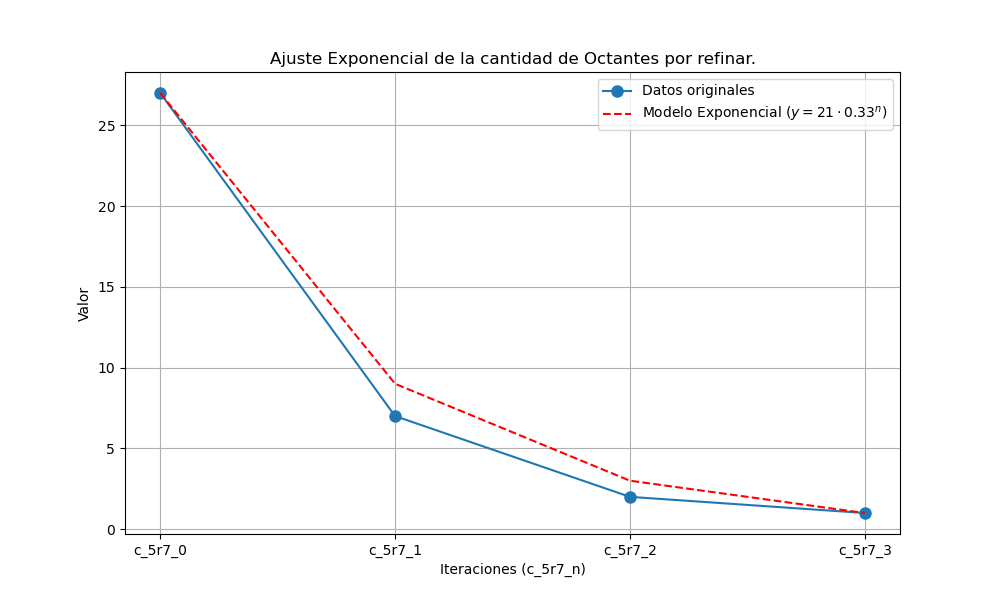
\includegraphics[width=1.0\textwidth]{figures/analysis/cortex/c_5r7_1_fit.png}
%		\end{subfigure}
%		\hfill
%		 \begin{subfigure}[t]{0.49\textwidth}
%			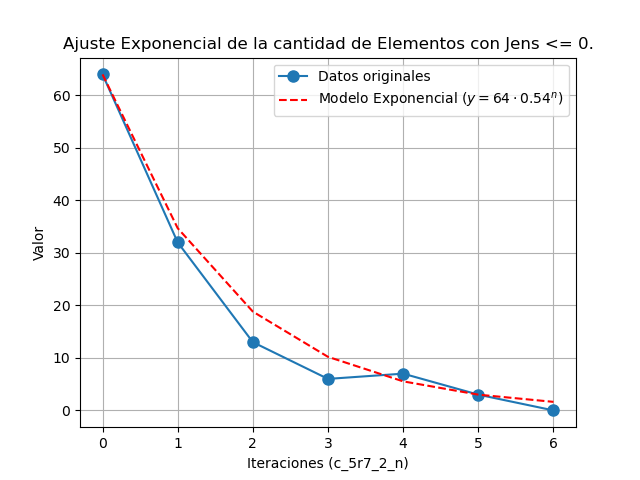
\includegraphics[width=1.0\textwidth]{figures/analysis/cortex/c_5r7_2_2_fit.png}
%		\end{subfigure}
%		\hfill
%		\begin{subfigure}[t]{0.49\textwidth}
%			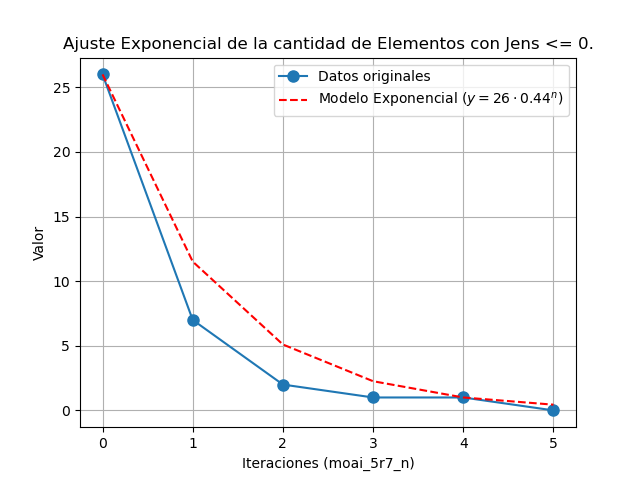
\includegraphics[width=1.0\textwidth]{figures/analysis/moai/moai_5r7_1_fit.png}
%		\end{subfigure}
%		\hfill
%		\begin{subfigure}[t]{0.49\textwidth}
%			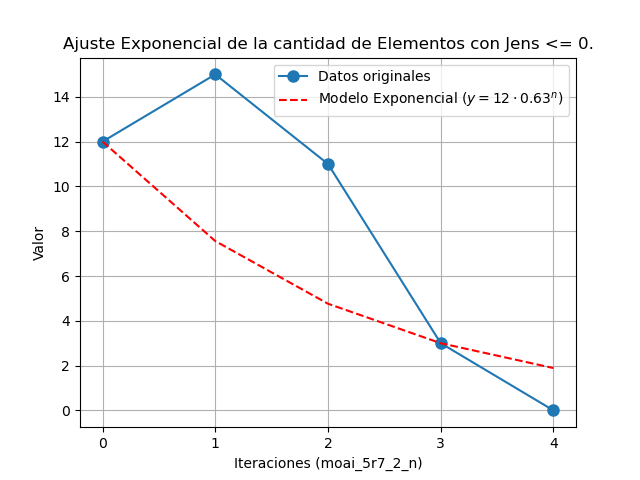
\includegraphics[width=1.0\textwidth]{figures/analysis/moai/moai_5r7_2_2_fit.png}
%		\end{subfigure}
%		\hfill
%		\begin{subfigure}[t]{0.49\textwidth}
%			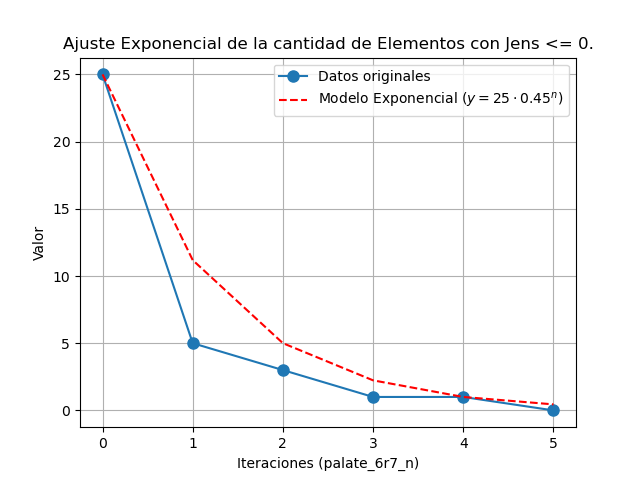
\includegraphics[width=1.0\textwidth]{figures/analysis/palate/palate_6r7_1_fit.png}
%		\end{subfigure}
%		\hfill
%		\begin{subfigure}[t]{0.49\textwidth}
%		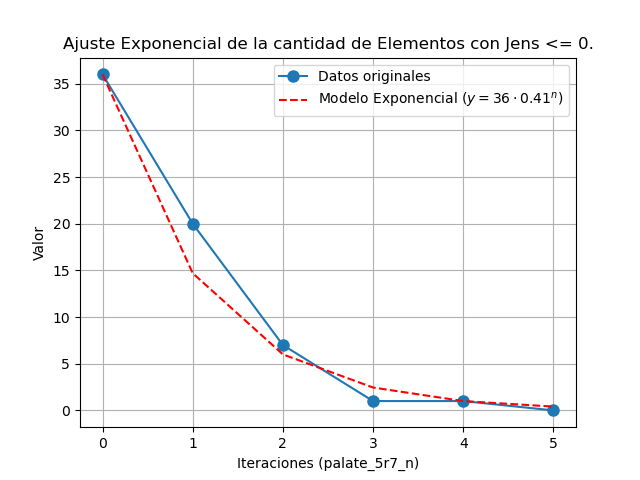
\includegraphics[width=1.0\textwidth]{figures/analysis/palate/palate_5r7_1_fit.png}
%		\end{subfigure}
%	\end{figure}
%		
%	\begin{figure}[!ht]
%		\ContinuedFloat
%		\centering
%		\begin{subfigure}[t]{0.49\textwidth}
%		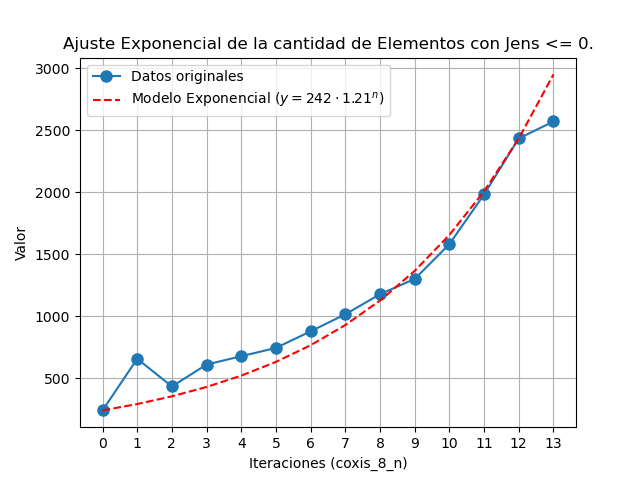
\includegraphics[width=1.0\textwidth]{figures/analysis/coxis/coxis_8_1_fit.png}
%		\end{subfigure}
%		\caption{ Representación Coxis sin refinamiento local. }
%		Fuente: Elaboración propia.
%		\label{fig:exponential_fit_all}
%	\end{figure}


	\begin{figure}[!ht]
		\centering
		\begin{subfigure}[t]{1.0\textwidth}
			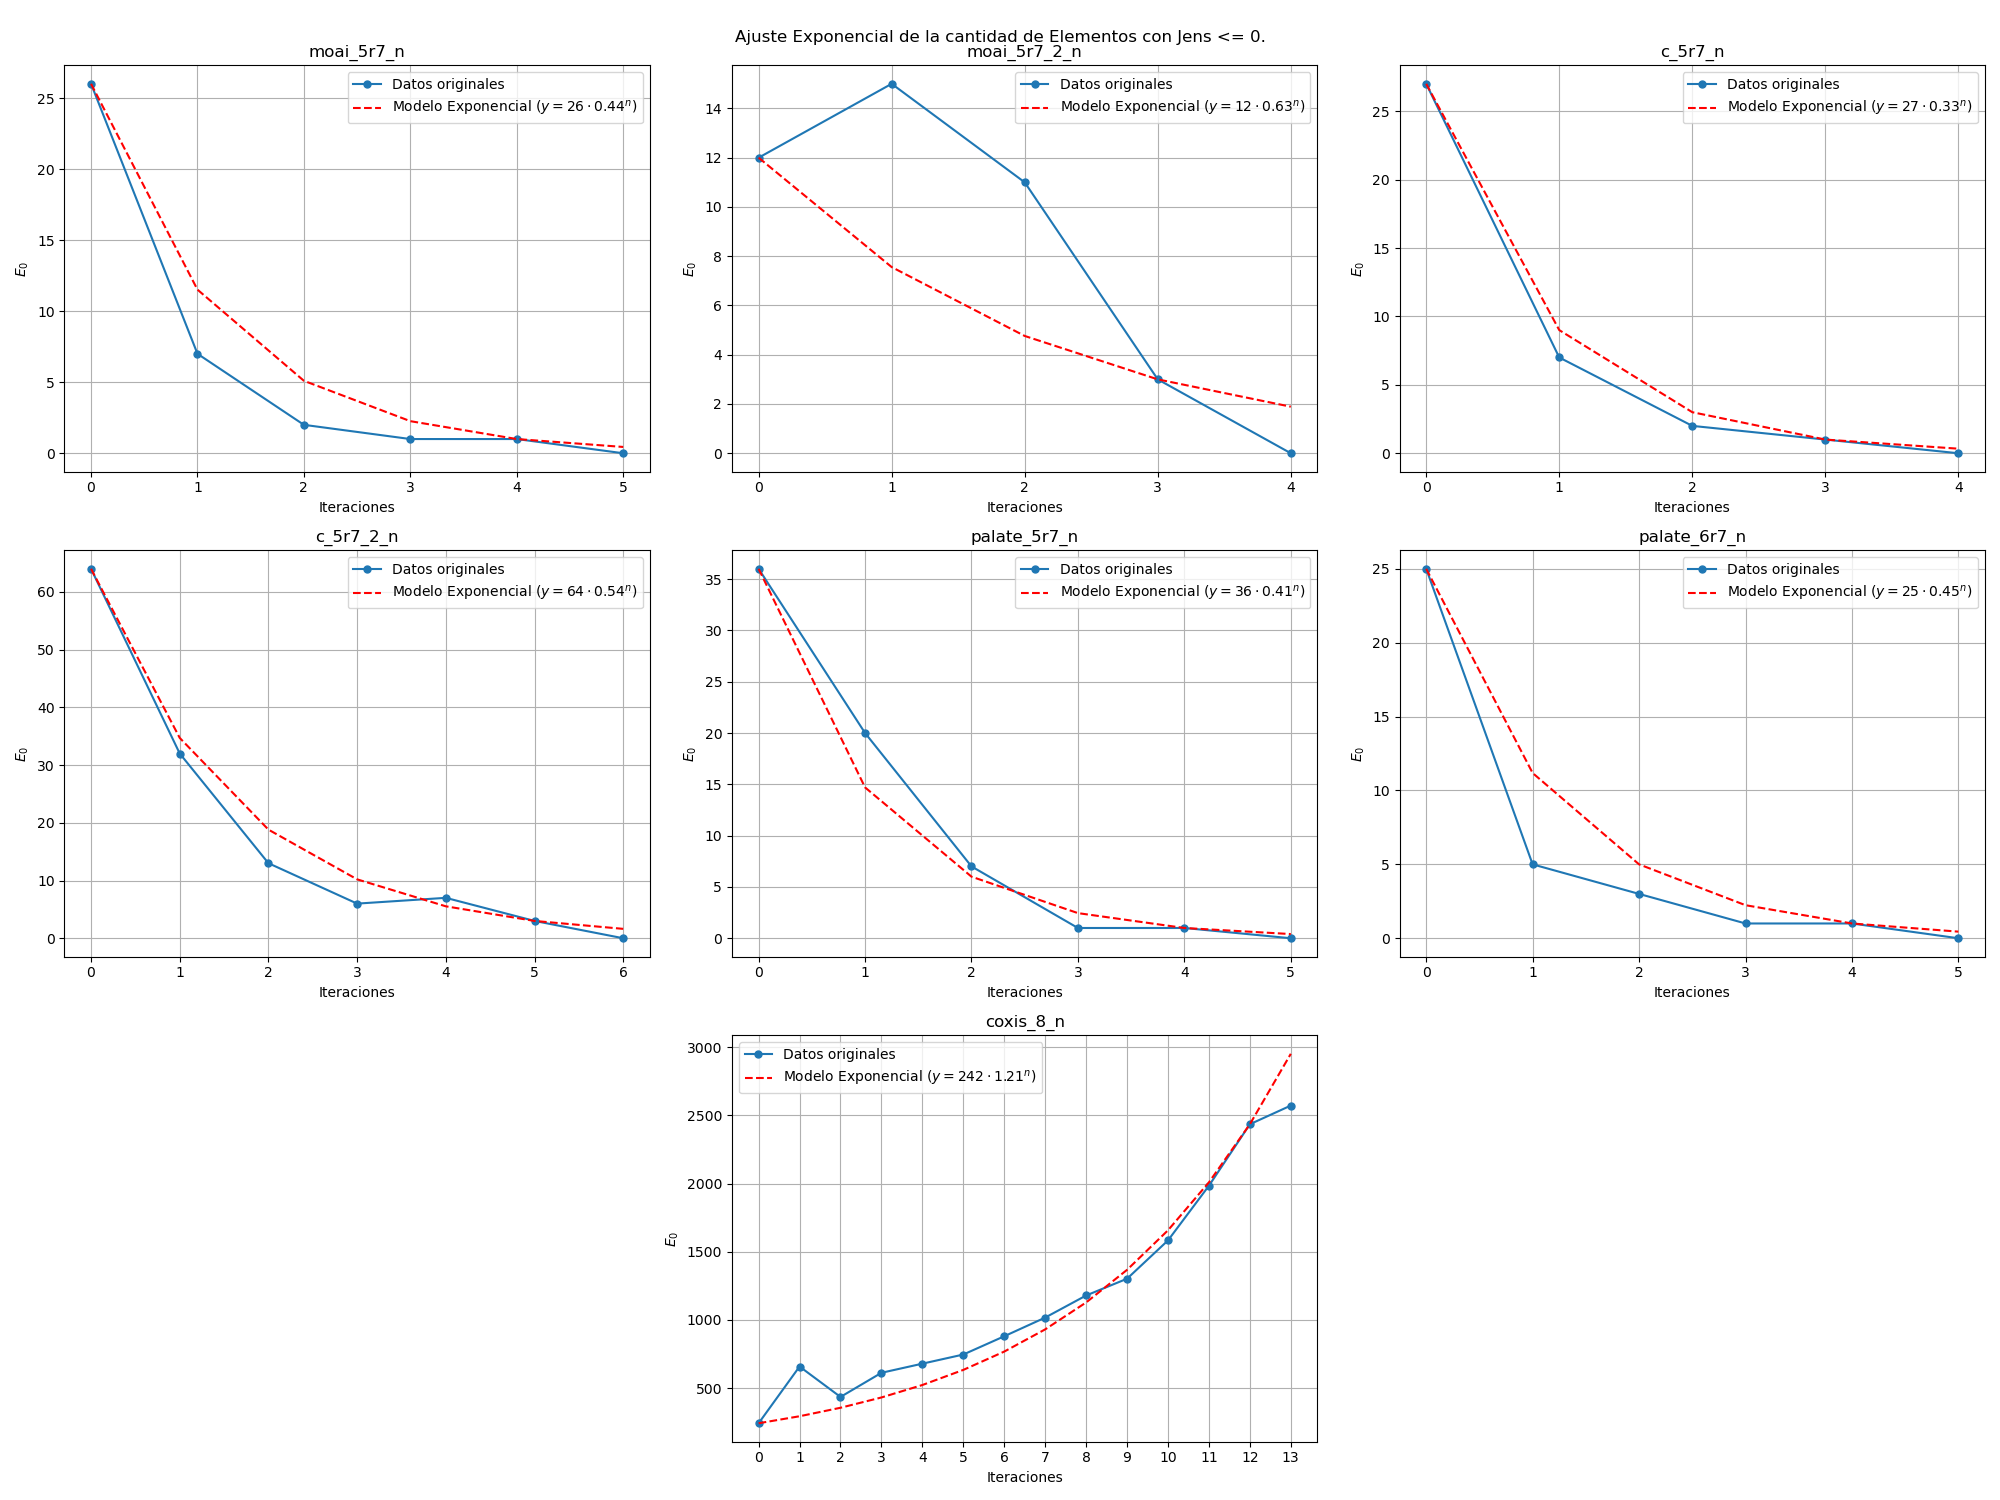
\includegraphics[width=0.75\paperheight, angle=90, origin=c]{figures/analysis/fit_all.png}
		\end{subfigure}
		\caption{ Ajuste exponencial de $E_0$ para todos los casos. }
		Fuente: Elaboración propia.
		\label{fig:exponential_fit_all}
	\end{figure}

\end{itemize}


\subsubsection{ Análisis del comportamiento de los Elementos posicionados en la vecindad a las zonas refinadas.}

Cuando se refina cada Octante con Elementos inválidos, genera una reacción en cadena de refinamiento en los Octantes adyacentes para mantener la consistencia en los niveles de refinamiento de la malla. Debe cumplirse que, dado un Octante $O$ con nivel de refinamiento $rl_o$, deben, sus vecinos directos, $\bar{O}$, tener un nivel de refinamiento $rl_{\bar{o}} \in \{rl_o + 1, rl_o - 1, rl_o\}$.


%La estadística $J_{ENS}$ se muestra como un histograma que representa la frecuencia de los Elementos $E_x$,  $\forall x \in \{0, 0.03, 0.05\}$, es decir, una función de frecuencia escalonada definiendo $x$ como las cota superiores de cada intervalo.

La estadística $J_{ENS}$ se muestra como un histograma que representa la frecuencia de Elementos, siendo este histograma una función de escalonada que define la frecuencia de Elementos de calidad deficiente. En \cite{shepherd-2008}, se define $J_{ENS_{SJ}} \in [0, 0.2[$, como Elementos cuestionables, es decir, Elementos de calidad deficiente. Además, destacar el estándar de ANSYS, que considera $J_{ENS_{AN}} \in [0, 0.03[$, como Elementos inválidos.

Por tanto, para este análisis se acotará definiendo $EC \in \{0, 0.03, 0.05\}$ como Elementos de calidad cuestionable.
Además, definiremos la frecuencia de Elementos con $J_{ENS} \in [m, n[$ , como $H^{n}_{m}$.

Entonces, se graficará en \autoref{fig:fit_all_bar}, los histogramas de cada malla para los intervalos definidos por $EC$.
Teniendo, $H^{0.0}_{-inf}$, $H^{0.03}_{0.0}$, $H^{0.05}_{0.03}$.

 $J_{ENS}$ con la frecuencia de $E_{EC} , \forall x \in \{0, 0.03, 0.05\}$

\begin{figure}[!ht]
	\centering
	\begin{subfigure}[t]{1.0\textwidth}
		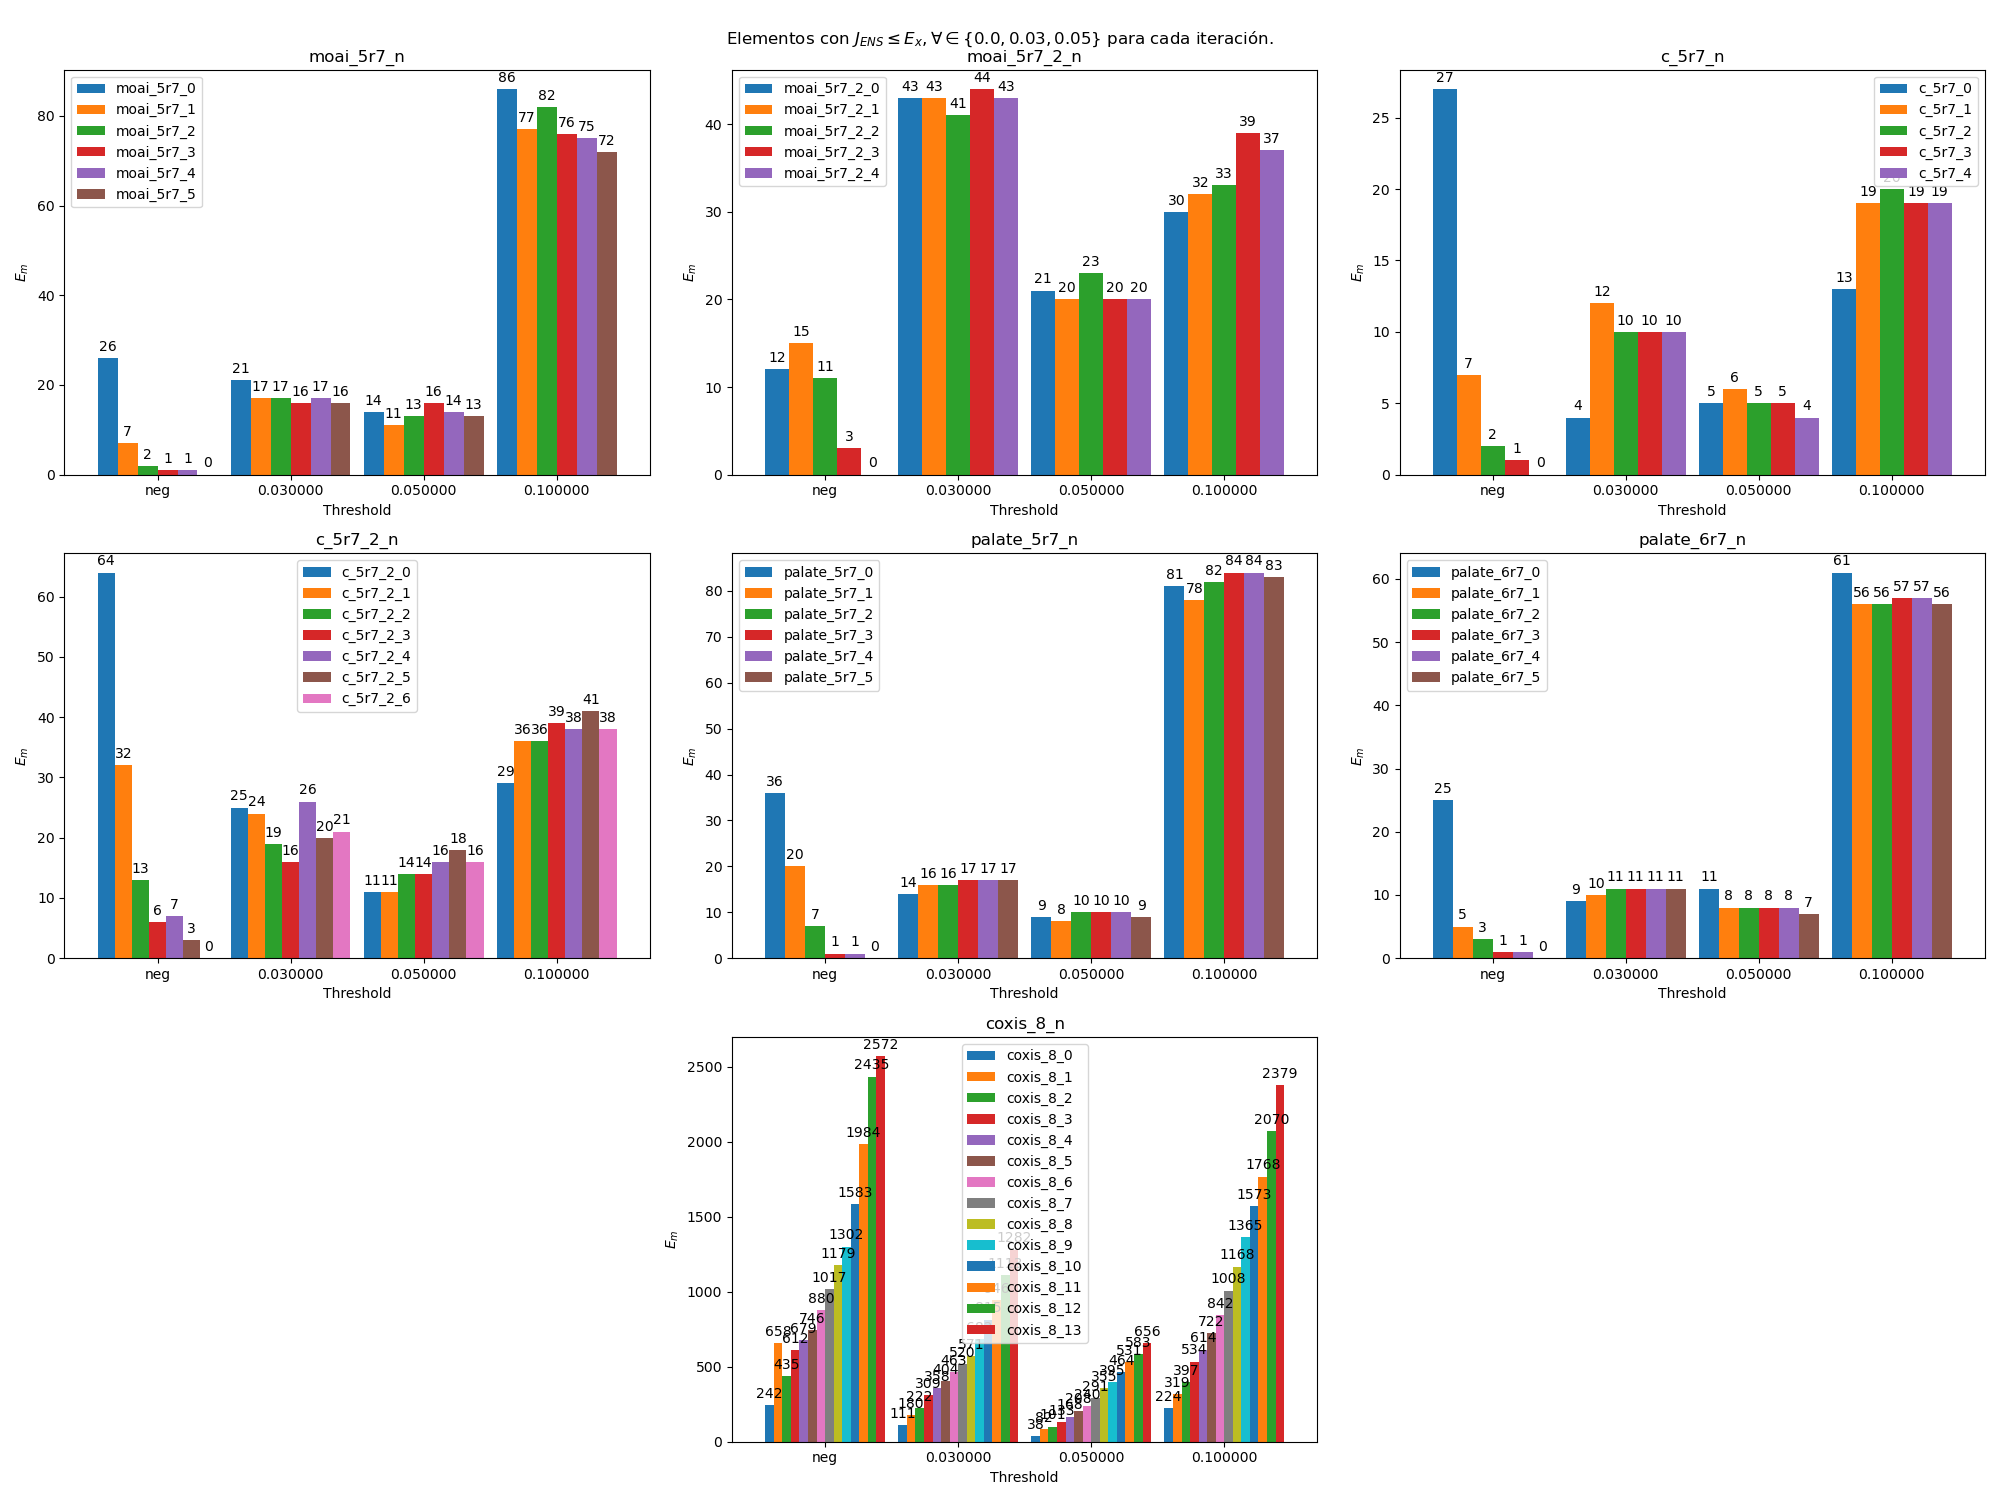
\includegraphics[width=0.75\paperheight, angle=90, origin=c]{figures/analysis/fit_all_bar.png}
	\end{subfigure}
	\caption{ Histograma agrupado por intervalo para todos los casos. }
	Fuente: Elaboración propia.
	\label{fig:fit_all_bar}
\end{figure}

